% https://tex.stackexchange.com/a/552328
\documentclass{beamer}
\mode<presentation>{\usetheme{Madrid}}

%%%%%%%%%%%%%%%%%%%%%%%%%%%%%%%%%%%%%%%%%%%%%%%%%%%%%%%%%%%%%%%%%%%%%%%%%%%%%%%%%%%%%%%%%%%%%%%%%%%%
\usepackage[style=verbose]{biblatex}
\bibliography{biblio}
\usepackage[utf8]{inputenc}
\usepackage{tikz}
\usetikzlibrary{shapes.geometric, arrows}
%%%%%%%%%%%%%%%%%%%%%%%%%%%%%%%%%%%%%%%%%%%%%%%%%%%%%%%%%%%%%%%%%%%%%%%%%%%%%%%%%%%%%%%%%%%%%%%%%%%%
\tikzstyle{startstop} = [rectangle, rounded corners, minimum width=3cm, minimum height=1cm,text centered, draw=black, fill=red!30]
\tikzstyle{io} = [trapezium, trapezium left angle=70, trapezium right angle=110, minimum width=3cm, minimum height=1cm, text centered, draw=black, fill=blue!30]
\tikzstyle{process} = [rectangle, minimum width=3cm, minimum height=1cm, text centered, text width=3cm, draw=black, fill=orange!30]
\tikzstyle{decision} = [diamond, minimum width=3cm, minimum height=1cm, text centered, draw=black, fill=green!30]
\tikzstyle{arrow} = [thick,->,>=stealth]
%%%%%%%%%%%%%%%%%%%%%%%%%%%%%%%%%%%%%%%%%%%%%%%%%%%%%%%%%%%%%%%%%%%%%%%%%%%%%%%%%%%%%%%%%%%%%%%%%%%%
\title[tikzpicture with beamer]{}

\begin{document}
\begin{frame}{tikzpicture}{}
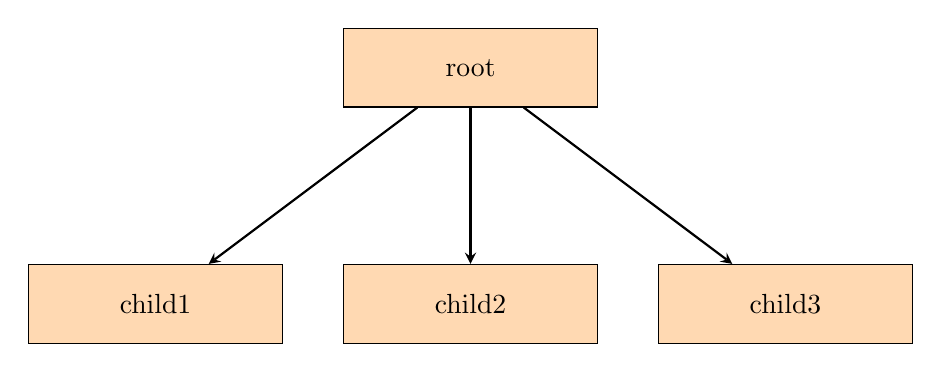
\begin{tikzpicture}[node distance=3cm]

\node (root) [process] {root};
\node (child1) [process, below of=root, xshift=-4cm] {child1};
\draw [arrow] (root) -- (child1);

\node<+(1)-> (child2) [process, below of=root, xshift=0cm] {child2};
\draw<.(1)-> [arrow] (root) -- (child2);

\node<+(1)-> (child3) [process, below of=root, xshift=4cm] {child3};
\draw<.(1)-> [arrow] (root) -- (child3);

\end{tikzpicture}   

\end{frame}

\end{document}
